% Fig. 2.22 / spec Fig A25 + A26 -- Jensen's inequality for a convex and for
%   a concave function, drawn for the two-point distribution
%   P(X = X_1) = P(X = X_2) = 1/2.
% Source: mathstatch2.tex lines 4170-4207 and 4216-4248, two separate
%   tikzpictures which spec 1.3 item 7 and the closing note of spec A26 both
%   require to become one picture sharing one x range, one y scale and one
%   axis length.
% 2026-08-08, by the author's ruling on CH2_INEQUALITY_AUDIT.md item B-11
%   (乙十一): the two panels now share ONE figure number, Fig. 2.22, which was
%   chosen over keeping two numbers and over splitting into two
%   separate figures on measured height (863.64 / 1148.51 px against
%   884.96 / 1172.51 and 953.69 / 1249.84, desktop / 390 px).  P221 carries
%   one <figure>, one <img> and a single caption; the anchor is
%   fig-jensen-convex, and the empty span that used to carry
%   fig-jensen-concave is gone.  The empirical-rule figure that follows in
%   P222 moved from Fig. 2.24 to Fig. 2.23, so the chapter now runs
%   Fig. 2.1 to 2.23.  Comments only -- no drawing command was touched.
%
% Functions, drawn on [0.15, 8.1] with samples=300:
%   convex   g(x) = 0.0784 (x - 2.3)^2 + 0.5
%   concave  h(x) = 2.8 - 0.0784 (x - 2.3)^2
% Two-point distribution X_1 = 0.6, X_2 = 7.6, each with probability 1/2, so
% E(X) = 4.1 is the midpoint of the two and E[g(X)] is the midpoint of the
% chord.  Every ordinate in the picture:
%   g(0.6) = 0.0784 x 1.7^2 + 0.5 = 0.226576 + 0.5 = 0.726576
%   g(7.6) = 0.0784 x 5.3^2 + 0.5 = 2.202256 + 0.5 = 2.702256
%   g(4.1) = 0.0784 x 1.8^2 + 0.5 = 0.254016 + 0.5 = 0.754016
%   chord midpoint (0.726576 + 2.702256)/2 = 3.428832/2 = 1.714416
%   h(0.6) = 2.8 - 0.226576 = 2.573424    h(7.6) = 2.8 - 2.202256 = 0.597744
%   h(4.1) = 2.8 - 0.254016 = 2.545984
%   chord midpoint (2.573424 + 0.597744)/2 = 3.171168/2 = 1.585584
% The gap the figure exists to show is the same on both panels:
%   1.714416 - 0.754016 = 0.9604 = 2.545984 - 1.585584
% which is the vertical dashed segment at x = 4.1 in each panel.  It has to
% be, since g + h = 3.3 is affine, so the two panels are one reflection of the
% other and E[g(X)] - g[E(X)] = h[E(X)] - E[h(X)] exactly.
%
% Deviations from CH2_FIGURE_SPECS.md:
%
% 1. Spec A25 and A26 record that the manuscript comments out both axes, so
%    E(X) has nothing to stand on and the two points at x = 4.1 are not joined
%    (spec 3.2 item 10).  Each panel here carries the x axis, ticks at 0.6,
%    4.1 and 7.6 labelled X_1, E(X), X_2, and a journalmuted dashed segment
%    joining (4.1, g[E(X)]) to (4.1, E[g(X)]).  The length of that segment is
%    the inequality, and the caption of P221 gives its value, 0.9604.
%
% 2. The manuscript draws the point (4.1, 2.545984) twice, one \node on top of
%    another (spec A26).  It is drawn once here; the duplicate is logged in
%    ERRATA and is not copied.
%
% 3. The manuscript's label offsets, +-0.5cm from each point with the node
%    centred, put the two labels at x = 4.1 about 0.1cm apart and run three of
%    the four boxes into the curve or off the left edge of the picture.  All
%    four are re-placed here (see the table below); the two at x = 4.1 are set
%    one above and one below, 1.85cm apart, against the 0.6cm of spec 1.3
%    item 5.  In the concave panel the label of (4.1, 2.545984) is the one
%    spec A26 singles out as fouling the top of the curve: it is set up and to
%    the right of its point, where the curve is already past its maximum at
%    x = 2.3 and falling away, so the box clears the curve by 0.24cm at its
%    binding corner and never comes near the crest.
%
% 4. The Chinese labels of the manuscript panels are gone, per spec 1.4;
%    convexity and concavity are named in the caption of P221.
%
% 5. The manuscript writes E for the expectation; the site writes \mathbb{E},
%    as the body text of P221 does.
%
% Placement of every text node.  With x = 0.885cm and y = 1.42cm, the 0.18cm
% of spec 1.3 item 5 is 0.2034 x-units and 0.1268 y-units, and a filled point
% of 3.6pt has radius 0.0446 y-units.  The clearances below are the ones
% measured back off the finished SVG, at the binding corner in each case:
%   convex   (X_1, g(X_1))   north west at (0.6, 0.3732): curve 0.187cm above
%                            the ink (its minimum 0.5 stands at x = 2.3,
%                            inside the box's span), axis 0.207cm below
%            (X_2, g(X_2))   south east at (7.6, 2.8736): point 0.19cm below,
%                            chord 0.268cm below, curve 0.302cm below
%            (E(X), g[E(X)]) north west at (4.1, 0.5827): point 0.187cm
%                            above, curve 0.268cm above, axis 0.504cm below
%            (E(X), E[g(X)]) south east at (4.1, 1.8857): point 0.187cm
%                            below, chord 0.268cm below
%            $g(x)$          north east at (8.1, 2.3809): curve 0.186cm above
%   concave  (X_1, h(X_1))   south west at (0.6, 2.9268): curve 0.187cm below
%            (X_2, h(X_2))   north east at (7.6, 0.4264): point 0.187cm
%                            above, chord 0.268cm above, axis 0.282cm below
%            (E(X), h[E(X)]) south west at (4.1, 2.7173): point 0.187cm
%                            below, curve 0.268cm below
%            (E(X), E[h(X)]) north east at (4.1, 1.4143): point 0.187cm
%                            above, chord 0.268cm above
%            $h(x)$          south east at (8.1, 0.9390): curve 0.203cm below
% The two labels at x = 4.1 stand 1.864cm apart in each panel, one above the
% chord and one below the curve, against the 0.6cm of spec 1.3 item 5.  Both
% curve labels sit against the last stretch of their own curve, on the side
% away from the chord, right-aligned with the end of the curve at x = 8.1;
% neither can go past it, since spec 1.3 item 4 keeps text inside the axis end
% at 8.2.  The tick labels stand 0.257cm below the axis, per the same item.
% The two panels share the window [0, 8.2] on x, one y unit and one axis
% length, and an unstroked \path pins each panel's window to [0, 3.25] on y so
% that the two are boxes of exactly one size; the tallest ink stands at 3.135
% in the convex panel and 3.155 in the concave one, so they also read at the
% same height.  The panels stand 0.49cm apart.
%
% Size and type.  Native 221.565 x 314.194 pt = 7.816 x 11.084 cm, inside the
% 9.0cm cap of spec 1.3.  The figure is a topic-figure--wide in body text,
% which .topic-figure--wide img sizes at min(100%, 620px), i.e. 350px in the
% 350px article column of a 390px phone.  A mark of S pt shows at
% S x 0.99626 x <display width> / 221.565 px, so
%     display width          350px (390px phone)      620px (desktop)
%     10pt text              15.74px                  27.88px
%      9pt \small            14.16px                  25.09px
%      8pt subscripts        12.59px                  22.30px
% The smallest marks in the picture are the 1 and the 2 of X_1 and X_2 inside
% the four \small point labels, at 8pt, i.e. 12.59px, above the 12px floor of
% spec 1.3.  \DeclareMathSizes{9}{9}{8}{7} is what puts them at 8pt: the
% default for 9pt text is a 7pt script, which would render at 11.0px and fail
% that floor.  No scriptscript size occurs.
\documentclass[tikz,border=2pt]{standalone}
\usepackage{amsmath}
\usepackage{amssymb}
\usepackage{xcolor}
\usetikzlibrary{arrows.meta}
\DeclareMathSizes{10}{10}{9}{8}
\DeclareMathSizes{9}{9}{8}{7}

\definecolor{journalink}{HTML}{1F1C18}
\definecolor{journalmuted}{HTML}{8A7F72}
\definecolor{journalaccent}{HTML}{9C2D2D}

\newcommand{\convexg}[1]{0.0784*(#1-2.3)*(#1-2.3)+0.5}
\newcommand{\concaveh}[1]{2.8-0.0784*(#1-2.3)*(#1-2.3)}

\begin{document}
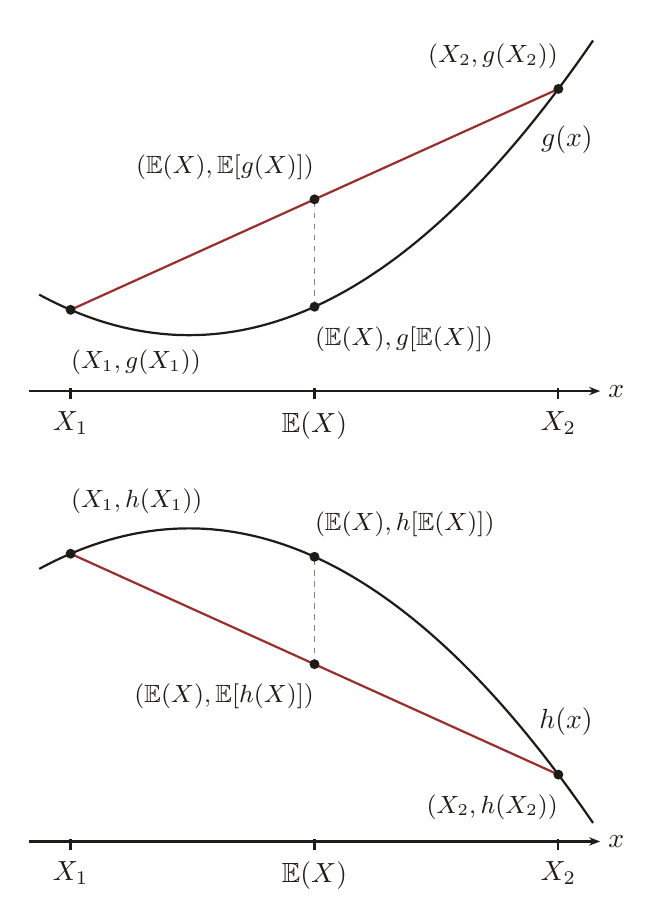
\begin{tikzpicture}[
  x=0.885cm,
  y=1.42cm,
  every node/.style={font=\normalsize, journalink},
  axis/.style={journalink, line width=0.8pt, -{Stealth[length=4pt]}},
  tick/.style={journalink, line width=0.8pt},
  curve/.style={journalink, line width=0.8pt},
  chord/.style={journalaccent, line width=0.8pt},
  guide/.style={journalmuted, line width=0.5pt, dash pattern=on 2pt off 2pt},
  dot/.style={circle, fill=journalink, inner sep=0pt, minimum size=3.6pt}
]

% =====================================================================
% upper panel of Fig. 2.22: convex g, E[g(X)] above g[E(X)]
% =====================================================================
\begin{scope}[yshift=0cm]
  % pin the panel window to [0, 3.25] on y, so both panels are boxes of one
  % size and the shared y range is exact rather than merely implied by the ink
  \path (0,0) (0,3.25);
  \draw[curve] plot[domain=0.15:8.1, samples=300, smooth]
    (\x,{\convexg{\x}});
  \draw[chord] (0.6,0.726576) -- (7.6,2.702256);
  \draw[guide] (4.1,0.754016) -- (4.1,1.714416);

  \draw[axis] (0,0) -- (8.2,0);
  \node[anchor=west, inner sep=2.8pt] at (8.2,0) {$x$};
  \foreach \p in {0.6, 4.1, 7.6}
    \draw[tick] ([yshift=0.035cm]\p,0) -- ([yshift=-0.106cm]\p,0);
  \node[anchor=north, inner sep=0pt] at ([yshift=-0.25cm]0.6,0) {$X_{1}$};
  \node[anchor=north, inner sep=0pt] at ([yshift=-0.25cm]4.1,0)
    {$\mathbb{E}(X)$};
  \node[anchor=north, inner sep=0pt] at ([yshift=-0.25cm]7.6,0) {$X_{2}$};

  \node[dot] at (0.6,0.726576) {};
  \node[dot] at (7.6,2.702256) {};
  \node[dot] at (4.1,0.754016) {};
  \node[dot] at (4.1,1.714416) {};

  \node[anchor=north west, inner sep=0pt] at (0.6,0.3732)
    {\small $(X_{1}, g(X_{1}))$};
  \node[anchor=south east, inner sep=0pt] at (7.6,2.8736)
    {\small $(X_{2}, g(X_{2}))$};
  \node[anchor=north west, inner sep=0pt] at (4.1,0.5827)
    {\small $(\mathbb{E}(X), g[\mathbb{E}(X)])$};
  \node[anchor=south east, inner sep=0pt] at (4.1,1.8857)
    {\small $(\mathbb{E}(X), \mathbb{E}[g(X)])$};

  \node[anchor=north east, inner sep=0pt] at (8.1,2.3809) {$g(x)$};
\end{scope}

% =====================================================================
% lower panel of Fig. 2.22: concave h, E[h(X)] below h[E(X)]
% =====================================================================
\begin{scope}[yshift=-5.72cm]
  \path (0,0) (0,3.25);
  \draw[curve] plot[domain=0.15:8.1, samples=300, smooth]
    (\x,{\concaveh{\x}});
  \draw[chord] (0.6,2.573424) -- (7.6,0.597744);
  \draw[guide] (4.1,1.585584) -- (4.1,2.545984);

  \draw[axis] (0,0) -- (8.2,0);
  \node[anchor=west, inner sep=2.8pt] at (8.2,0) {$x$};
  \foreach \p in {0.6, 4.1, 7.6}
    \draw[tick] ([yshift=0.035cm]\p,0) -- ([yshift=-0.106cm]\p,0);
  \node[anchor=north, inner sep=0pt] at ([yshift=-0.25cm]0.6,0) {$X_{1}$};
  \node[anchor=north, inner sep=0pt] at ([yshift=-0.25cm]4.1,0)
    {$\mathbb{E}(X)$};
  \node[anchor=north, inner sep=0pt] at ([yshift=-0.25cm]7.6,0) {$X_{2}$};

  \node[dot] at (0.6,2.573424) {};
  \node[dot] at (7.6,0.597744) {};
  \node[dot] at (4.1,2.545984) {};
  \node[dot] at (4.1,1.585584) {};

  \node[anchor=south west, inner sep=0pt] at (0.6,2.9268)
    {\small $(X_{1}, h(X_{1}))$};
  \node[anchor=north east, inner sep=0pt] at (7.6,0.4264)
    {\small $(X_{2}, h(X_{2}))$};
  \node[anchor=south west, inner sep=0pt] at (4.1,2.7173)
    {\small $(\mathbb{E}(X), h[\mathbb{E}(X)])$};
  \node[anchor=north east, inner sep=0pt] at (4.1,1.4143)
    {\small $(\mathbb{E}(X), \mathbb{E}[h(X)])$};

  \node[anchor=south east, inner sep=0pt] at (8.1,0.9390) {$h(x)$};
\end{scope}

\end{tikzpicture}
\end{document}
